\documentclass{article}

\usepackage{amsmath,amssymb}
\usepackage{graphicx}
\usepackage{array}
\usepackage[margin=1in]{geometry}
\usepackage{dsfont}

% ===== This makes my \affil cmnd work.
\usepackage[affil-it]{authblk}


% ===== This makes my environments work switching llncs to article.
\newtheorem{theorem}{Theorem}[section]
\newtheorem{lemma}[theorem]{Lemma}
\newtheorem{proposition}[theorem]{Proposition}
\newtheorem{corollary}[theorem]{Corollary}

\newenvironment{proof}[1][Proof]{\begin{trivlist}
\item[\hskip \labelsep {\bfseries #1}]}{\end{trivlist}}
\newenvironment{definition}[1][Definition]{\begin{trivlist}
\item[\hskip \labelsep {\bfseries #1}]}{\end{trivlist}}
\newenvironment{example}[1][Example]{\begin{trivlist}
\item[\hskip \labelsep {\bfseries #1}]}{\end{trivlist}}
\newenvironment{remark}[1][Remark]{\begin{trivlist}
\item[\hskip \labelsep {\bfseries #1}]}{\end{trivlist}}

\newcommand{\qed}{\nobreak \ifvmode \relax \else
      \ifdim\lastskip<1.5em \hskip-\lastskip
      \hskip1.5em plus0em minus0.5em \fi \nobreak
      \vrule height0.75em width0.5em depth0.25em\fi}

% ===== For \algorithm. Is this a decent idea?
\usepackage[lined,boxed,ruled,vlined]{algorithm2e}

% ===== For \mathscr
\usepackage{mathrsfs}
\DeclareSymbolFontAlphabet{\mathrsfs}{rsfs}
\usepackage[mathscr]{eucal}


% ===== For \boldsymbol
\usepackage{amsbsy}

% ===== For \bm (bold math)
\usepackage{bm}

\usepackage{fixltx2e}
\MakeRobust{\overrightarrow}

% ===== For code snippets
\usepackage{courier}

% ==== Misha and Ning's Notation file =====
%% ----------------------------------------------------------------------
%% Definitions, Macros, Etc.
%% ----------------------------------------------------------------------

%% Hyper-linked References
\newcommand{\Sec}[1]{\hyperref[sec:#1]{\S\ref*{sec:#1}}} %section
\newcommand{\Eqn}[1]{\hyperref[eq:#1]{(\ref*{eq:#1})}} %equation
\newcommand{\Fig}[1]{\hyperref[fig:#1]{Figure~\ref*{fig:#1}}} %figure
\newcommand{\Tab}[1]{\hyperref[tab:#1]{Table~\ref*{tab:#1}}} %table
\newcommand{\Thm}[1]{\hyperref[thm:#1]{Theorem~\ref*{thm:#1}}} %theorem
\newcommand{\Lem}[1]{\hyperref[lem:#1]{Lemma~\ref*{lem:#1}}} %lemma
\newcommand{\Prop}[1]{\hyperref[prop:#1]{Property~\ref*{prop:#1}}} %property
\newcommand{\Cor}[1]{\hyperref[cor:#1]{Corollary~\ref*{cor:#1}}} %corollary
\newcommand{\Def}[1]{\hyperref[def:#1]{Definition~\ref*{def:#1}}} %definition
\newcommand{\Alg}[1]{\hyperref[alg:#1]{Algorithm~\ref*{alg:#1}}} %algorithm
\newcommand{\Ex}[1]{\hyperref[ex:#1]{Example~\ref*{ex:#1}}} %example

% Theorem-like constructs
%\newtheorem{example}[theorem]{Example}

% Blackboard fonts 
\newcommand{\Real}{\mathbb{R}}
\newcommand{\Cplx}{\mathbb{C}}
%% Transposes
\newcommand{\Tra}{^{\rm T}} % Transpose
\newcommand{\Cct}{^\dagger} % Complex conjugate transpose

%% Permutation index
\newcommand{\bfpp}{{\bf p}_n}

%% Matrix & Tensor Operations
\newcommand{\Circ}[1]{{\rm circ}\left( #1 \right)}
\newcommand{\Fold}[1]{{\rm fold}\left( #1 \right)}
\newcommand{\Unfold}[1]{{\rm unfold}\left( #1 \right)}
\newcommand{\Twist}[1]{{\rm twist}(\M{#1})}
\newcommand{\Squeeze}[1]{{\rm squeeze}(#1)}
\newcommand{\squeeze}{{\rm squeeze}}
\newcommand{\Mout}{\diamondsuit}
\newcommand{\circu}{ {\rm circ}}
\newcommand{\bcirc}{ {\rm circ}}
\newcommand{\vvec}{ {\rm vec}}

\newcommand{\mc}[1]{\mathcal{#1}}
\newcommand{\mb}[1]{\mathbb{#1}}
\newcommand{\mcr}[1]{\mathrsfs{#1}}

%% Element of complicated object that is surrounded by parens
\newcommand{\PE}[2]{\left( #1 \right)_{#2}}

%% Vector notation
\newcommand{\V}[1]{{\bm{\mathbf{\MakeLowercase{#1}}}}} % vector
\newcommand{\VE}[2]{\MakeLowercase{#1}_{#2}} % vector element

%% Matrix notation
\newcommand{\M}[1]{{\bm{\mathbf{\MakeUppercase{#1}}}}} % matrix
\newcommand{\Mhat}[1]{{\bm{\hat \mathbf{\MakeUppercase{#1}}}}} % matrix
\newcommand{\Mbar}[1]{{\bm{\bar \mathbf{\MakeUppercase{#1}}}}} % matrix
\newcommand{\ME}[2]{\MakeLowercase{#1}_{#2}} % matrix element
\newcommand{\MC}[2]{\V{#1}_{#2}}

%% Tensor notation
\newcommand{\T}[1]{\boldsymbol{\mathscr{\MakeUppercase{#1}}}} %tensor
\newcommand{\TLS}[2]{\M{#1}_{[#2]}} % lateral slice
\newcommand{\TFS}[2]{\M{#1}_{#2}} % frontal slice
\newcommand{\TT}[2]{\V{#1}_{#2}} % tube
\newcommand{\TE}[2]{\MakeLowercase{#1}_{#2}} % tensor element


%% Shortcuts
\newcommand{\TA}{\T{A}}
\newcommand{\TB}{\T{B}}
\newcommand{\TS}{\T{S}}
\newcommand{\TC}{\T{C}}
\newcommand{\TU}{\T{U}}
\newcommand{\TV}{\T{V}}
\newcommand{\TG}{\T{G}}

\newcommand{\Vu}{\V{u}}
\newcommand{\Vv}{\V{v}}
\newcommand{\Vq}{\V{q}}
\newcommand{\Vr}{\V{r}}
\newcommand{\Vp}{\V{p}}
\newcommand{\Vd}{\V{d}}
\newcommand{\Vz}{\V{z}}
\newcommand{\Vb}{\V{b}}
\newcommand{\Vg}{\V{g}}
\newcommand{\Vh}{\V{h}}
\newcommand{\MH}{\M{H}}
\newcommand{\MG}{\M{G}}
\newcommand{\MA}{\M{A}}
\newcommand{\MX}{\M{X}}
\newcommand{\MZ}{\M{Z}}
\newcommand{\MW}{\M{W}}
%\newcommand{\TD}{\T{D}}

\newcommand{\SaS}{{\mathcal S}}

\newcommand{\MGC}{\tilde{\MG}}

\newcommand{\Matlab}{{\sc Matlab}\xspace}
\newcommand{\matlab}{{\sc Matlab}\xspace}
\newcommand{\qtext}[1]{\quad\text{#1}\quad}

\newcommand{\matvec}{{\tt Vec}}
\newcommand{\fld}{{\tt Fold}}

\def \bK{\mathbf{K}}
\def \bF{\mathbf{F}}
\def \bD{\mathbf{D}}
\def \bB{\mathbf{B}}
\def \bA{\mathbf{A}}
\newcommand{\bDelta}{\boldsymbol{\Delta}}

%\newcommand{\bea}{\left[ \begin{array}}
%\newcommand{\eea}{ \end{array} \right]} 

\newcommand{\bftheta}{ {\boldsymbol \theta}}
\newcommand{\bfrho}{ {\boldsymbol \rho}}
\newcommand{\bfeta}{ {\boldsymbol \eta}}
\newcommand{\fft}{ \mbox{\tt fft} }
\newcommand{\ifft}{ \mbox{\tt ifft} }
\newcommand{\blkd}{\mbox{\tt blkdiag}}
\newcommand{\rshpT}{\mbox{\tt reshapeT}}
\newcommand{\F}[1]{\mathcal{F}\{#1\}}
\newcommand{\Fi}[1]{\mathcal{F}^{-1}\{#1\}}
\newcommand{\indep}{\perp\!\!\!\perp}

\usepackage{mathtools}
\DeclarePairedDelimiter{\ceil}{\lceil}{\rceil}
\DeclarePairedDelimiter{\floor}{\lfloor}{\rfloor}
\newcommand{\Var}{\text{Var}}
\newcommand{\E}{\text{E}}
\newcommand{\Cov}{\text{Cov}}



%%%% Dr. K's colored comments. 
\usepackage{color} 
\definecolor{blue}{rgb}{0,0,1}
\definecolor{red}{rgb}{1,0,0}
\definecolor{purple}{rgb}{1,0,1}
\newcommand\MEK[1]{\textcolor{red}{MEK: #1}}
\newcommand\EMK[1]{\textcolor{purple}{EMK: #1}}
\newcommand\SA[1]{\textcolor{blue}{SA: #1}}

\begin{document}



Eric Kernfeld

Summary of Wilkinson's ``Parameter inference for stochastic kinetic models of bacterial gene regulation'', a book chapter in \cite{Bernardo2012}.

\section{Purpose}
This paper develops tools to study bacterial behavior, which is sometimes nondeterministic. It investigates a possible mechanism for this randomness: fluctuations in biochemical systems that regulate cell metabolism. In other papers, these systems are modeled using continuous-time Markov jump processes. This gives a rigorous treatment of stochastic dynamics. One remaining issue is parameter inference from data that are noisy, discrete-time, and partial. The paper addresses this problem via Bayesian inference and MCMC.

\section{Bare-Bones Biology}
 As a motivating case, Wilkinson uses the ``decision'' of {\it Bacillus subtilis} whether to become mobile. The paper centers around a gene encoding {\it flagellin}, which is a protein component of organelles that allow motility. Because it can be disorienting, I'll relay some of the biological relationships in short sentences in the next paragraph. 

The protein {\it flagellin} helps bacteria move. The protein $\sigma^D$ promotes {\it flagellin}. The {\it fla / che} operon \footnote{Operons are the basic transistor-like elements of the genome. In response to an outside stimulus, such as high levels of the sugar lactose, a normally active operon may become inactive or vice versa. By ``active'', I mean that the DNA encoded by the operon can be transcribed into RNA.} contains many motility-related genes, including the one for $\sigma^D$. The protein $\sigma^A$ and the protein {\it CodY} both suppress the {\it fla / che} operon. Thus, they suppress $\sigma^D$, and they indirectly suppress {\it flagellin}. In fact, {\it CodY} also downregulates {\it flagellin} directly. This is easiest to digest as a figure.

\begin{figure}[h!]
\begin{center}
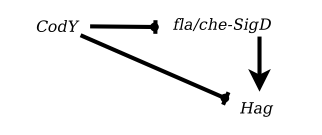
\includegraphics[scale=0.5]{wilkinson_reg_network.png}
\caption{Regulatory relationships. $Hag$ is the gene for $flagellin$, while $SigD$ encodes $\sigma^D$.}
\end{center}
\label{fig:}
\end{figure}


%Rather than describing regulatory relations in sentences, I'll relay Wilkinson's biochemical highlights in the following table. 
%
%$\left[
%\begin{tabular}{ >{}c<{} >{}c<{} >{}c<{} >{$}c<{$}}
% Name & Type of Molecule & suppresses & promotes& Is suppressed by & Is promoted by\\
% 
%flagellin & protein & -- & -- & -- & $\sigma^D$, {\it CodY} \\
%%
% $\sigma^D$ & protein & -- & -- & -- & -- \\
%%
% $\sigma^A$ & protein & -- & -- & -- & -- \\
%%
% {\it CodY}  & Type of Molecule & suppresses & promotes& Is suppressed by & Is promoted by\\
%\end{tabular} 
%\right]$
\EMK{Editing note: for consistency, fix every expression where $\theta$ is to the left of $x$.}

\section{The Model}
Since we're simulating a biochemical system, suppose there are $X_{j}(t)$ particles of type $j$ at time $t$, $j\in \{1 ... u\}$. These particles interact via a set of reactions $\mathcal{R}_i$, $i\in \{1 ... v\}$, with $\mathcal{R}_i$ consuming $p_{ij}$ particles of type $j$ and producing $q_{ij}$ particles of type $j$. I'll refer to these en masse as $X(t)$, $P$, $Q$ and once it $R_i(t)$ is defined, $R(t)$. Defining the matrix $S$ to be $Q^T-P^T$, and letting $R_{i}(t)$ denote the number of reactions of type $i$ in $[0,t]$, then $X(t) - X(0) = SR(t)$. Under some assumptions, the different reaction channels evolve independently, and $R_i(t)$ is a Poisson process with intensity $c_i\int_0^t \prod_{j=1}^u {{X_j(t)}\choose{p_{ij}}}$. %Define $h_i(c_i, X(t)) \equiv c_i\int_0^t \prod_{j=1}^u {{X_j(t)}\choose{p_{ij}}}$. 
The $c_i$'s are unknown.

Suppose $n$ reactions occur between time $0$ and time $T$. Suppose the $i$th one occurs at time $t_i$ and suppose it has type $\nu_i$. Define $t_0\equiv0$ and $t_{n+1}\equiv T$. When it comes to inference, you may recognize the likelihood as a competing hazards model from continuous Markov chain theory\footnote{At times, I choose to use equations that stand free of sentences. These I do not punctuate.}. \EMK{This likelihood is a guess, because Wilkinson writes it using a function ($h_0$) that he never defines. Working for now on the fact that they're competing (homogeneous) Poisson processes. I'm fairly sure this is correct as I have it, or in other words, that $h_0$ is $\sum h_i$.}
$$P(\nu, t|c) = \prod_{i=1}^n c_{\nu_i} \prod_{j=1}^u {{X_{j}(t_{i-1})}\choose{p_{{\nu_i}j}}}\exp(-c_{\nu_i}\int_0^T {{X_j(t)}\choose{p_{{\nu_i}j}}} )dt$$

Wilkinson points out that $\int_0^T {{X_j(t_{i-1})}\choose{p_{{\nu_i}j}}}dt$ is tractable; in fact, it is $\sum_{i=0}^{n} (t_{i+1}-t_{i}) {{X_j(t_{i})}\choose{p_{{\nu_i}j}}}$. 

If the number of reactions of type $k$ is $r_k$, then the likelihood becomes 
$$P(\nu, t|c) = \prod_{k=1}^u \left\{ c_{k}^{r_k} 
\left\{\prod_{j=1}^u { X_{j}(t_{i-1})\choose p_{kj}}^{r_k}\right\}\exp(-c_{k}\int_0^T \sum_j{X_j(t)\choose p_{kj}} )dt\right\}.$$  
Still calling it the likelihood, Wilkinson omits the bracketed term $\prod_{j=1}^u { X_{j}(t_{i-1})\choose p_{kj}}^{r_k}$, probably because it does not involve $c$. Either way, the gamma distribution is conjugate for $c_k$, and setting independent priors $c_k\sim \Gamma(a_k, b_k)$, the posteriors are independent with $c_k\sim \Gamma(a_k+r_k, b_k+\int_0^T \sum_j {X_j(t) \choose p_{kj}}dt )$. This is an ideal scenario; missing data make inference more challenging.

\section{Inference}

In Wilkinson's data, not every reaction is recorded. Measurements are intermittent, and only some of the particle counts are measured. There is error in the measurements, to boot.  The tidy scheme above scheme falls to pieces. Wilkinson says it better than I can: ``Consider first the best-case scenario--perfect observation of the system at discrete times. Conditional on discrete-time observations, the Markov process breaks up into a collection of independent bridge processes that appear not to be analytically tractable.'' He goes on to mention alternative strategies, which include the MCMC scheme of \cite{Boys2008} and the approximation \cite{gillespie_CLE_2000} paired with inference via \EMK{cite more Wilkinson papers here.}

%For my own benefit: to produce a chain of samples from $P(\theta|D)$, using a proposal $q(\theta^*|\theta)$, accept with probability $\min \{1, A\}$ if $A=\frac{q(\theta|\theta^*)}{q(\theta^*|\theta)} \times \frac{P(\theta^*|D)}{P(\theta|D)}$. 

The crux of the paper is a new competitor to all of these. It builds upon the fact that exact simulations from this model are possible, and also on the fact that measurement error helps soften the requirements on where the bridge should begin and end. Let $\theta$ include $c$, controlling the reaction rates, and $\tau$, controlling the degree of measurement error. Let $x$ denote the true state of the chain, but measured only at discrete times. That means the likelihood $P(x|\theta)$ is thought to be intractable. Let $\mathcal{D}$ be $x$ measured with error and possibly with missing data for some particle types. 

If we want to construct a Metropolis-Hastings scheme to sample a new value $(x^*, \theta^*)$ from $P(x, \theta|\mathcal{D})=P( \theta)P(x| \theta)P(\mathcal{D}|x, \theta)$ using a proposal $f(\theta^*, x^*|\theta, x)$, it works out that the acceptance ratio must be the min of 1 and $\frac{f(\theta^*, x^*|\theta, x)}{f(\theta, x|\theta^*, x^*)}\times \frac{ P( \theta)}{ P( \theta^*)} \times \frac{P(x| \theta)}{P(x^*| \theta^*)} \times \frac{P(\mathcal{D}|x, \theta)}{P(\mathcal{D}|x^*, \theta^*)}$. In the model Wilkinson considers, $P(\mathcal{D}|x,\theta)$ is simple, but $P(x|\theta)$ is not feasible to compute. The insight is that one can cancel the term $ \frac{P(x| \theta)}{P(x^*| \theta^*)}$ by constructing a proposal that contains  $\frac{P(x^*| \theta^*)}{P(x| \theta)}$ as a factor. This spills straight out if instead of drawing both $x$ and $\theta$ from out-of-the-box proposals, we draw $\theta^*\sim f(\theta^*|\theta)$ and compute $x^*$ via simulation with parameters $\theta^*$. The end result is that the ratio of interest simplifies:
\begin{align*}
&\frac{f(\theta^*, x^*|\theta, x)}{f(\theta, x|\theta^*, x^*)}\times \frac{P(x| \theta)}{P(x^*| \theta^*)}\times \frac{ P( \theta)}{ P( \theta^*)}  \times \frac{P(\mathcal{D}|x, \theta)}{P(\mathcal{D}|x^*, \theta^*)}\\
&=\frac{f(\theta^*|\theta)}{f(\theta|\theta^*)}\times \frac{P(x^*| \theta^*)}{P(x| \theta)} \times \frac{P(x| \theta)}{P(x^*| \theta^*)} \times \frac{ P( \theta)}{ P( \theta^*)}\times \frac{P(\mathcal{D}|x, \theta)}{P(\mathcal{D}|x^*, \theta^*)}\\
&=\frac{f(\theta^*|\theta)}{f(\theta|\theta^*)}\times \frac{ P( \theta)}{ P( \theta^*)}\times \frac{P(\mathcal{D}|x, \theta)}{P(\mathcal{D}|x^*, \theta^*)}.
\end{align*}
To simplify further, use an independence sampler with the prior as a proposal and your calculation reduces to $ \frac{P(\mathcal{D}|x, \theta)}{P(\mathcal{D}|x^*, \theta^*)}.$

If the measurement error is small, or $\mathcal{D}$ is high-dimensional, or both, this scheme leads to very high rejection rates, so it is not usable. Instead, you can break down $X$ and $\mathcal{D}$ over time and use an M-H step that alters only one coordinate of $x$. %This relies on the fact that the hidden state sequence is Markovian, i.e. that $P(x, \theta|\mathcal{D}) = \prod_t P(x_{t+1}, \theta|x_t, \mathcal{D})P(x_t, \theta|\mathcal{D})$. 
 Suppose you draw inputs from $P(\theta, x|\mathcal{D}_{1:t})$, propose $(\theta^*, x_t^*)$ by perturbing $(\theta, x_t)$ slightly, and propose $x_{t+1}^*$ with a new forward simulation. Suppose you then accept with probability $\min\{1,
\frac{P(\mathcal{D}_{t+1}|x_{t+1}^*, \theta^*)}{P(\mathcal{D}_{t+1}|x_{t+1}, \theta)}\}$. The claim is that you are left with an exact draw from $P(\theta, x|\mathcal{D}_{1:t+1})$. \EMK{Why is this true? This doesn't quite seem to match any of the schemes discussed in 516. It seems to be sequential monte carlo, which I'm now trying to teach myself.} This leads to higher acceptance rates, and by starting with the prior and moving up through time, you arrive at samples from the posterior conditioned on all the data.

%The proposal ratio $\times$ posterior ratio can be expanded as $$
%\frac{P(x_{t+1}^*| x_t^*,\theta^*, \mathcal{D}_t)}{P(x_{t+1}| x_t^*, \theta, \mathcal{D}_t)} 
%\frac{P(x_t^*,\theta^*| \mathcal{D}_t)}{P(\theta,x_t| \mathcal{D}_t)}
%\times 
%\frac{P(x_{t+1}^*| \theta, x_t)}{P(x_{t+1}| x_t^*,\theta^*)}  
%\frac{ P( \theta,x_t)}{ P( x_t^*,\theta^*)}   
%\frac{P(\mathcal{D}_t|x_t, \theta)}{P(\mathcal{D}_t|x_t^*, \theta^*)}.$$ That shows 

At this point, Wilkinson describes a connection to Approximate Bayesian Computation (ABC), and he describes software and computing tools that can be used to run the model. 

\section{An experiment}
Wilkinson next describes a twelve-reaction regulatory model for these chemicals, spelling it out in table 1, and he lists three known reaction rates that can be used to test the model's performance. The prior distributions are each log-uniform over 4 orders of magnitude. The experiment assumes $D_t$ is the number of $\sigma^D$ molecules observed with Gaussian error s.d. 10 molecules. The initial state of the cell is assumed known, and observations occur every 5 minutes for 2 hours. Wilkinson says ``1,000,000 particles were used, together with a burn-in of 1,000 iterations and a thin of 5[.]'' \EMK{He never defines particles, so pending further reading, my best guess is that this means he starts with 1e6 samples from the prior, carrying each one forward. Not sure how the burn-in fits in.} 

He also repeats this experiment, altering the measurement process so that it relies on a proxy for $\sigma^D$, a fluorescent protein (GFP). He performs inference by a) plugging GFP levels into the algorithm as if they were exactly proportional to $\sigma^D$ and b) including the production and decay of GFP in the biochemical model. He concludes that plugging in GFP for $\sigma^D$ leads to strong, incorrect posteriors, but that the full model is still useful.

\section{Extensions}
Wilkinson mentions many areas for future work. 
\begin{itemize}
\item His likelihood-free MCMC scheme applies to any hidden, discretely observed continuous Markov process. It also can be used for multiple time-series $\mathcal{D}^1, ..., \mathcal{D}^p$ by using posteriors from one as priors for the next.
\item This method can fuse data from two bacterial strains, one missing a certain gene, by using posteriors from one experiment as priors for the next. It can also accomodate multiple fluorescent ``reporters'' for different molecules.
\item Unsolved problems include scaling the method up to process data on batches of cells observed en masse and integrating data from microarrays or RNA-seq.
\end{itemize}


\begin{align*}
\end{align*}
\begin{align*}
\end{align*}
\begin{align*}
\end{align*}
\begin{align*}
\end{align*}

%\texttt{code snippet}
%
%\begin{algorithm}[h]
%\caption{ }
%Do things\\
%Loop:\\
%\Indp
% Do this again and again\\
%\end{algorithm}

%\begin{figure}[h!]
%\begin{center}
%\includegraphics[height=4in,width=6in]{filename.pdf}
%\caption{}
%\end{center}
%\label{fig:}
%\end{figure}

%$\left[
%\begin{tabular}{ >{$}c<{$} >{$}c<{$}}
% 1 & -\phi_1\\
% -\phi_1 & 1
%\end{tabular} 
%\right]$

%==== Bib files and style =======
\bibliographystyle{splncs}
\bibliography{prelim_biblio}
\end{document}
